\documentclass{article}
\usepackage{graphicx}
\usepackage{amsmath}
\usepackage{pgfplots}
\usepackage{array}
\usepackage[margin=1.5cm]{geometry}
\usepackage{adjustbox}
\usepackage{hyperref}
\usepackage{cite}
\usepackage{listings}
\usepackage{xcolor}
\usepackage{comment}
\usepackage{graphicx}
\usepackage{pdfpages}
\usepackage{enumitem}
\usepackage{pgfplotstable}
\usepackage{booktabs}
\usepackage{adjustbox}
\usepackage{changepage}
\usepackage[utf8]{inputenc}
\lstset{ 
literate= {á}{{\'a}}1 
    {é}{{\'e}}1 
    {í}{{\'i}}1 
    {ó}{{\'o}}1 
    {ú}{{\'u}}1
} 

\hypersetup{
colorlinks=true,
linkcolor=blue,
urlcolor=blue,
}

\pgfplotsset{compat=1.17}
\usepackage[portuguese]{babel}

\definecolor{codegreen}{rgb}{0,0.6,0}
\definecolor{codegray}{rgb}{0.5,0.5,0.5}
\definecolor{codepurple}{rgb}{0.58,0,0.82}
\definecolor{backcolour}{rgb}{0.95,0.95,0.92}

\lstdefinestyle{mystyle}{
    backgroundcolor=\color{backcolour},   
    commentstyle=\color{codegreen},
    keywordstyle=\color{magenta},
    numberstyle=\tiny\color{codegray},
    stringstyle=\color{codepurple},
    basicstyle=\ttfamily\footnotesize,
    breakatwhitespace=false,         
    breaklines=true,                 
    captionpos=b,                    
    keepspaces=true,                 
    numbers=left,                    
    numbersep=5pt,                  
    showspaces=false,                
    showstringspaces=false,
    showtabs=false,                  
    tabsize=2
}

\lstset{style=mystyle}

\title{Projeto Final de Análise Numérica}
\author{Alisson Cordeiro e Gabriel Gaspar}
\date{}

\begin{document}

\maketitle

\section{Introdução}
\paragraph{} Este projeto tem como objetivo apresentar o estudo de Interpolação Polinomial, para a matéria de Análise Númerica, do 3° semestre do curso de Ciência da Computação do Instituto Federal do Paraná - Campus Pinhais. A Interpolação Polinomial é uma técnica utilizada para encontrar um polinômio que passa por um conjunto de pontos dados, permitindo a estimativa de valores intermediários e a análise do comportamento da função.

\section{Código-fonte}
\lstinputlisting[language=c++]{code/main.cpp}

\section{Utilização do programa}
\paragraph{} Para compilar e utilizar o programa, foi usado o seguinte código:

\begin{lstlisting}[language=bash]
    g++ -o interpola interpola.cpp
\end{lstlisting}

Para uso do programa, foi usado um arquivo de entrada, contendo os valores necessários, sendo o primeiro valor, a quantidade de pontos conhecidos e o restante sendo os pares ordenados representando os pontos. Um exemplo de entrada está disponível abaixo, em \hyperref[sec:resultados]{Resultados}.

\begin{lstlisting}[language=bash]
    ./interpola < entrada.txt
\end{lstlisting}

A saída do programa está de acordo com as especificações do trabalho, com os valores sendo exibidos em ordem crescente do grau da variável, sendo o primeiro valor referente a \( x^0 \), seguido por \( x^1 \), \( x^2 \), até \( x^{n-1} \).

\newpage
\section{Resultados}
\label{sec:resultados}
\paragraph{} Usando a tabela abaixo como entrada, o número 5 representa a quantidade de pontos e o resto são os pontos em si. Com isso, o programa retorna a função abaixo da tabela.

\begin{table}[h!]
\centering
\begin{tabular}{cc}
\multicolumn{2}{c}{5} \\
1   & 2 \\
1.3 & 4.4 \\
1.7 & 4.56 \\
1.9 & 5 \\
2.3 & 7 \\
\end{tabular}
\end{table}

\begin{equation*}
f(x) = -10{,}561661x^4 + 77{,}710623x^3 - 207{,}739316x^2 + 241{,}080037x - 98{,}489683
\end{equation*}

A figura abaixo mostra o gráfico da função interpoladora, com os cinco pontos previamente dados plotados sobre ele para verificar o ajuste:

\begin{figure}[h!]
    \centering
    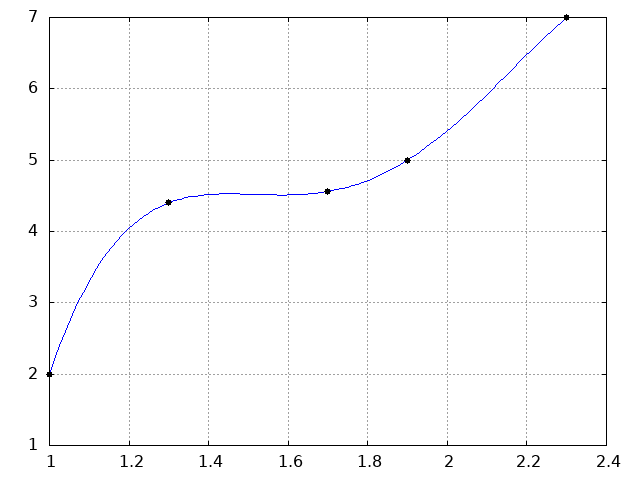
\includegraphics[width=0.5\linewidth]{saida.png}
    \caption{Gráfico da função com os pontos dados previamente}
    \label{fig:saida}
\end{figure}




\end{document}